\documentclass[border=20pt]{standalone}

\usepackage{tikz}
\usepackage{ifthen}
\usetikzlibrary{arrows, positioning, calc}
\usetikzlibrary{shapes.multipart} 

\newcommand{\inputTikZ}[2]{\scalebox{#1}{\subfile{#2}}}


\usepackage{subfiles}
\usepackage{standalone}
\def\tkzscl{1}
\newcommand{\smeq}{\medmuskip=0mu \thickmuskip=0mu \thinmuskip=0mu}


\begin{document}
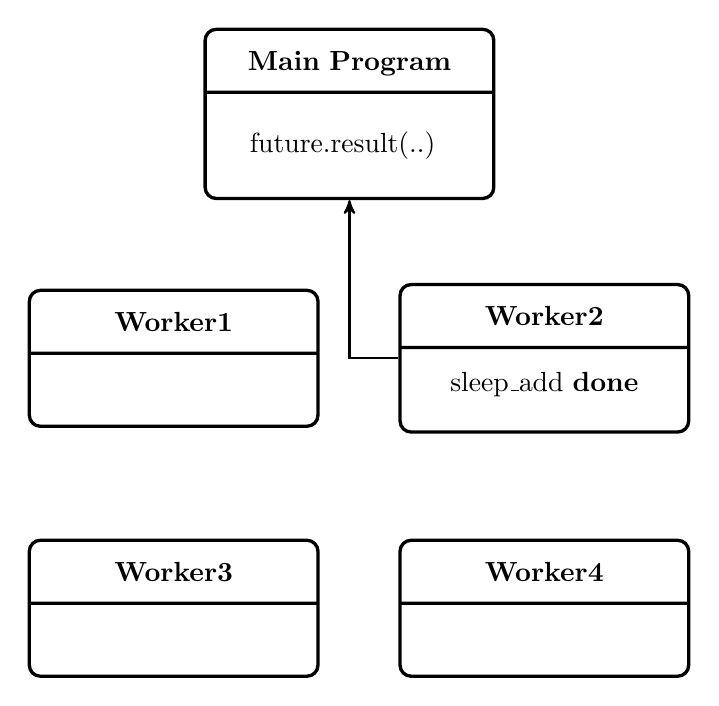
\begin{tikzpicture}[scale=\tkzscl]
\def\step{5}
\def\stylesub{\ifthenelse{\step=1}{white}{black}}

\tikzset{
    %Define standard arrow tip
    >=stealth',
    %Define style for boxes
    worker/.style={
    		text width=10em,
    		align=center,
			rectangle,
			fill=white,
			rounded corners,
			draw=black, very thick,
			rectangle split,
			rectangle split parts=2,
			inner sep=.5ex,
			text height=2.8ex, text depth=1.2ex,
			rectangle split part align=base,
			},
    subworker/.style={
    		worker,
    		draw=black,
    		text=black
			},
    second/.style={
           text height=2.8ex, text depth=1.2ex,
           text centered},
    pil/.style={
           ->,
           thick,
           %shorten <=2pt,
           %shorten >=2pt,}
    }
};

\node[worker] (main) {\bf Main Program\nodepart{second} \phantom{sleep}\\
\ifthenelse{\step=1}{sleep\_add}{
\ifthenelse{\step=2}{sleep\_add}{
\ifthenelse{\step=3}{submit(..)}{
\ifthenelse{\step=4}{future}{
\ifthenelse{\step=5}{future.result(..)}{
\ifthenelse{\step=6}{res}}}}}}
\phantom{}\\\phantom{sleep}
};
\node[left=6em of main.south] (a) {};
\node[subworker, below=of a] (w1) {\bf Worker1\nodepart{second} \phantom{sleep}\phantom{sleep}\\\phantom{sleep}}; 
\node[subworker, right=of w1] (w2) {\bf Worker2\nodepart{second} 
\ifthenelse{\step<3}{\phantom{sleep}\phantom{sleep}\\\phantom{sleep}}{
\ifthenelse{\step=3}{\phantom{.}\phantom{.}\\sleep\_add \\\phantom{.}}{
\ifthenelse{\step=4}{\phantom{.}\phantom{.}\\sleep\_add(..)\\\phantom{.}}{
\ifthenelse{\step=5}{\phantom{.}\phantom{.}\\sleep\_add \bf done\\\phantom{.}}{
\phantom{sleep}\phantom{sleep}\\\phantom{sleep}}}}}

}; 
\node[subworker, below=4em of w1] (w3) {\bf Worker3\nodepart{second} \phantom{sleep}\phantom{sleep}\\\phantom{sleep}}; 
\node[subworker, right=of w3] (w4) {\bf Worker4\nodepart{second} \phantom{sleep}\phantom{sleep}\\\phantom{sleep}};

\ifthenelse{\step=3}{\draw[pil] (main.south) |- (w2.west);}{}
\ifthenelse{\step=5}{\draw[pil] (w2.west) -| (main.south);}{}
%

% Draw a centered plus sign



\end{tikzpicture}
\end{document}